% import packages
\documentclass[8pt,handout,table=xcolor]{beamer}
\usepackage[utf8]{inputenc}
\usepackage{colortbl}
\usepackage{ragged2e}
\usepackage{booktabs}
\usepackage{threeparttable}
\usepackage{graphicx}
\usepackage{hhline}
\usepackage{amsmath}
\usepackage{amssymb}
\usepackage{amsthm}
\usepackage{tikz}
\usepackage{bm}
\usepackage[export]{adjustbox}
\usepackage[justification=centering]{caption}
\usepackage[backend=bibtex,style=authoryear,maxcitenames=2,natbib=true,maxbibnames=99]{biblatex}

% set beamer parameters
\usetheme{Frankfurt}
\usecolortheme{default}
\setbeamerfont{footnote}{size=\Tiny}
\setbeamertemplate{page number in head/foot}{}
\setbeamertemplate{bibliography item}{}
\setbeamertemplate{caption}[numbered]
\setbeamercovered{transparent}
\setbeamerfont{institute}{size=\small}
\addtobeamertemplate{navigation symbols}{}{%
  \usebeamerfont{footline}%
  \usebeamercolor[fg]{footline}%
  \hspace{2em}%
  \raisebox{1.7pt}[0pt][0pt]{\insertframenumber/\inserttotalframenumber}
}
\setbeamertemplate{enumerate items}[square]
\setbeamertemplate{section in toc}[square]
\setbeamertemplate{theorems}[numbered]

% special command to uncover graphics
% source: https://tex.stackexchange.com/a/415335
\newcommand<>{\uncovergraphics}[2][{}]{
  % Taken from: <https://tex.stackexchange.com/a/354033/95423>
  \begin{tikzpicture}
    \node[anchor=south west,inner sep=0] (B) at (4,0)
    {\includegraphics[#1]{#2}}; \alt#3{}{%
      \fill [draw=none, fill=white, fill opacity=0.7] (B.north west) -- (B.north
      east) -- (B.south east) -- (B.south west) -- (B.north west) -- cycle; }
  \end{tikzpicture}
}

% set caption parameters
\DeclareCaptionFormat{myformat}{\fontsize{6}{6}\selectfont#1#2#3}
\captionsetup{format=myformat}
\captionsetup[figure]{labelfont={bf},name={Figure}}
\captionsetup[table]{labelfont={bf},name={Table}}

% set bibliography parameters
\renewcommand\refname{Bibliography}
\addbibresource{../bibtex.bib}
\setlength\bibitemsep{1.5\itemsep}
\let\oldcitep=\citep
\renewcommand\citep[1]{{\textcolor{blue}{\oldcitep{#1}}}}
\let\oldcitet=\citet
\renewcommand\citet[1]{{\textcolor{blue}{\oldcitet{#1}}}}

% miscellaneous settings
\settowidth{\leftmargini}{\usebeamertemplate{itemize item}}
\addtolength{\leftmargini}{\labelsep}
\renewcommand{\arraystretch}{1.3}
\graphicspath{{../visuals/}}
\newcolumntype{L}[1]{>{\RaggedRight\hspace{0pt}}p{#1}}

% set admin details
\title{SoPa++: Leveraging explainability from hybridized RNN, CNN and weighted
  finite-state neural architectures}
\subtitle{M.Sc. Thesis Defense}
\author{Atreya Shankar (799227), \texttt{shankar.atreya@gmail.com} \\ Cognitive Systems:
  Language, Learning, and Reasoning (M.Sc.) \\ 1\textsuperscript{st} Supervisor: Dr. Sharid
  Loáiciga, University of Potsdam \\ 2\textsuperscript{nd}
  Supervisor: Mathias Müller, M.A., University of Zurich}
\institute{Foundations of Computational Linguistics \\ Department of Linguistics \\ University of Potsdam, SoSe 2021}
\date{July 8, 2021}

% start presentation
\begin{document}
\begin{frame}
  \maketitle
\end{frame}

\begin{frame}
  \frametitle{Overview}
  \tableofcontents
\end{frame}

\section{Introduction}

\begin{frame}
  \frametitle{Motivation}

  \begin{columns}[T]
    \begin{column}{.40\textwidth}
      \begin{itemize}
        \setlength\itemsep{1em}
        \uncover<1>{
          \item Trend of increasingly complex deep learning models achieving
          SOTA performance on ML and NLP tasks (Figure \ref{fig:nlp_progress})
          \item To address emerging concerns such as inductive biases, several
          studies make arguments for research into XAI; for example
          \citet{danilevsky2020survey} and \citet{arrieta2020explainable}}
        \uncover<2>{
          \item \citet{schwartz2018sopa} approach XAI in NLP by proposing an
          explainable hybridized neural architecture called \textbf{So}ft
          \textbf{Pa}tterns (SoPa; Figure \ref{fig:sopa_crop})
          \item SoPa provides \textbf{localized} and \textbf{indirect} explainability despite
          being suited for globalized and direct \textbf{explanations by
          simplification}
        }
      \end{itemize}
    \end{column}
    \hfill
    \begin{column}{.60\textwidth}
        \centering
        \uncovergraphics<1>[width=6cm, valign=t]{pdfs/borrowed/nlp_sota_model_size_progress.pdf}
        \uncover<1>{\captionof{figure}{Parameter counts of recently released pre-trained language
            models; figure taken from \citet{sanh2019distilbert}}}
        \label{fig:nlp_progress}
        \vspace{10pt}
        \uncover<2>{\fbox{\uncovergraphics<2>[width=6cm, valign=t]{pdfs/borrowed/sopa_crop.pdf}}}
        \uncover<2>{\captionof{figure}{Excerpt from \citet{schwartz2018sopa}}}
        \label{fig:sopa_crop}
    \end{column}
  \end{columns}
\end{frame}

\begin{frame}
  \frametitle{Objective and research questions}

  \uncover<1->{ Objective: \setlength{\leftmargini}{0.5cm}
    \begin{itemize}
      \item Address limitations of SoPa by proposing \textbf{SoPa++}, which
      could allow for effective explanations by simplification.
    \end{itemize}
  }
  
  \vspace{10pt}

  \uncover<2->{ Process:
    \begin{itemize}
      \item We study the performance and explanations by simplification of
      SoPa++ on the Facebook Multilingual Task Oriented Dialog (\textbf{FMTOD}) data set from
      \citet{schuster-etal-2019-cross-lingual}; focusing on the English-language
      intent classification task.
    \end{itemize}
  }
  
  \vspace{10pt}

  \uncover<3->{ Research questions:
    \begin{enumerate}
      \setlength\itemsep{1em}
      \item Does SoPa++ provide \textbf{competitive} performance?
      \item To what extent does SoPa++ contribute to \textbf{effective}
      explanations by simplification?
      \item What \textbf{interesting and relevant} explanations can SoPa++
      provide?
    \end{enumerate}
  }
\end{frame}

% macro for showing TOC on each new section
\AtBeginSection[]
{
  \begin{frame}
    \frametitle{Overview}
    \tableofcontents[currentsection]
  \end{frame}
}

\section{Background concepts}

\begin{frame}
  \frametitle{Explainability}
  \begin{columns}[T]
    \begin{column}{.40\textwidth}
      \begin{itemize}
        \setlength\itemsep{1em}
        \uncover<1>{
          \item Transparency is a passive feature that a model exhibits
          \item Explainability is an active feature that involves target
          audiences (Figure \ref{fig:xai_target_audience})
          \item \citet{arrieta2020explainable} explore a taxonomy of post-hoc
          explainability techniques}
        \uncover<2>{
          \item Explainability techniques can provide meaningful insights into
          decision boundaries within black-box models (Figure
          \ref{fig:lime_husky})
          \item Prominent explainability techniques include local
          explanations, feature relevance and \textbf{explanations by
            simplification}
        } 
      \end{itemize}
    \end{column}
    \hfill
    \begin{column}{.60\textwidth}
        \centering
        \uncovergraphics<1>[width=6.2cm,trim={0.3cm 0.3cm 0.5cm
          0.3cm},clip,valign=t]{pdfs/borrowed/xai_target_audience.pdf}
        \uncover<1>{\captionof{figure}{Examples of various target audiences in XAI; figure taken from
            \citet{arrieta2020explainable}}}
        \label{fig:xai_target_audience}
        \vspace{5pt}
        \uncovergraphics<2>[width=6cm,trim={0.1cm 0.1cm 0.1cm
          0.1cm},clip,valign=t]{pdfs/borrowed/lime_husky.pdf}
        \uncover<2>{\captionof{figure}{Local explanation for ``Wolf''
            classification decision, figure taken from \citet{lime}}}
        \label{fig:lime_husky}
    \end{column}
  \end{columns}
\end{frame}

\begin{frame}
  \frametitle{SoPa: Weighted Finite-State Automaton (WFA)}
  \uncover<1>{\begin{definition}[Semiring; \citealt{kuich1986linear}]
      \label{def:semiring}
      A semiring is a set $\mathbb{K}$ along with two binary associative
      operations $\oplus$ (addition) and $\otimes$ (multiplication) and two
      identity elements: $\bar{0}$ for addition and $\bar{1}$ for
      multiplication. Semirings require that addition is commutative,
      multiplication distributes over addition, and that multiplication by
      $\bar{0}$ annihilates, i.e., $\bar{0} \otimes a = a \otimes \bar{0} =
      \bar{0}$.

      \begin{itemize}
        \item Semirings follow the following generic notation: $\langle
        \mathbb{K}, \oplus, \otimes, \bar{0}, \bar{1} \rangle$.
        \item \textbf{Max-sum} semiring: $\langle \mathbb{R} \cup \{-\infty\},
        \text{max}, +, -\infty, 0 \rangle$
        \item \textbf{Max-product} semiring: $\langle \mathbb{R}_{>0} \cup
        \{-\infty\}, \text{max}, \times, -\infty, 1 \rangle$
      \end{itemize}
    \end{definition}}

  \uncover<2>{\begin{definition}[Weighted finite-state automaton;
      \citealt{peng2018rational}]
      \label{def:wfa}
      A weighted finite-state automaton over a semiring $\mathbb{K}$ is a
      5-tuple $\mathcal{A} = \langle \Sigma, \mathcal{Q}, \bm{\Gamma},
      \bm{\lambda}, \bm{\rho} \rangle$, with:

      \begin{itemize}
        \itemsep0em
        \item[--] a finite input alphabet $\Sigma$;
        \item[--] a finite state set $\mathcal{Q}$;
        \item[--] transition matrix $\bm{\Gamma}: \mathcal{Q} \times \mathcal{Q}
        \times (\Sigma \cup \{\epsilon\}) \rightarrow \mathbb{K}$;
        \item[--] initial vector $\bm{\lambda}: \mathcal{Q} \rightarrow
        \mathbb{K}$;
        \item[--] and final vector $\bm{\rho}: \mathcal{Q} \rightarrow
        \mathbb{K}$.
      \end{itemize}
    \end{definition}}
\end{frame}

\begin{frame}
  \frametitle{SoPa: Computational graph}
  \centering
  \captionsetup{width=9cm}
  \uncovergraphics<1>[width=8cm, valign=t]{pdfs/generated/generic_nfa_linear_chain/main.pdf}
  \uncover<1>{\captionof{figure}{WFA slice: linear-chain FA with
      self-loop (blue), $\epsilon$ (red) and main-path (black) transitions; figure
      adapted from \citet{schwartz2018sopa}}}
  \label{fig:fa}
  \vspace{10pt}
  \uncovergraphics<2>[width=8cm, valign=t]{pdfs/borrowed/sopa_computational_graph.pdf}
  \uncover<2>{\captionof{figure}{SoPa's partial computational graph; figure taken from
      \citet{schwartz2018sopa}}}
  \label{fig:sopa}
\end{frame}

\begin{frame}
  \frametitle{SoPa: Post-hoc explainability techniques}
    \begin{columns}[T]
    \begin{column}{.40\textwidth}
      \begin{itemize}
        \setlength\itemsep{1.4em}
        \uncover<1>{
          \item SoPa provides two post-hoc explainability techniques; namely
          \textbf{local explanations} and \textbf{feature relevance}
          \item Local explanations gather highest scoring phrases across the
          training data (Figure \ref{fig:sopa_local_explanations})
          }
        \uncover<2>{
          \item Feature relevance perturbs inputs using an occlusion technique
          to determine the highest impact phrases for a classification decision
          (Figure \ref{fig:sopa_feature_relevance})
          \item Overall, both techniques are \textbf{localized} and
          \textbf{indirect}
          \item WFAs have a rich theoretical background which can be exploited
          for more direct and globalized explanations
        }
      \end{itemize}
    \end{column}
    \hfill
    \begin{column}{.60\textwidth}
      \centering
      \uncovergraphics<1>[width=6cm,valign=t]{pdfs/borrowed/sopa_local_explanations.pdf}
      \uncover<1>{\captionof{figure}{Ranked local explanations from SoPa;
          table taken from \citet{schwartz2018sopa}}}
      \label{fig:sopa_local_explanations}
      \vspace{5pt}
      \uncovergraphics<2>[width=6cm,trim={0cm 2.3cm 0cm
        0cm},clip,valign=t]{pdfs/borrowed/sopa_feature_relevance.pdf}
      \uncover<2>{\captionof{figure}{Feature relevance outputs from SoPa;
          table taken from \citet{schwartz2018sopa}}}
      \label{fig:sopa_feature_relevance}
    \end{column}
  \end{columns}
\end{frame}

\section{Data and methodologies}

\begin{frame}
  \frametitle{FMTOD: Summary statistics}
  \begin{table}
    \small
    \centering
    \begin{threeparttable}
      \begin{tabular}{llll}
        \toprule
        Class and description & Frequency & Utterance length$^{\dagger}$ & Example$^{\ddagger}$ \\
        \midrule
        0: \texttt{alarm/cancel\_alarm} & \cellcolor{red!5}1791 & 5.6 $\pm$ 1.9 & cancel weekly alarm \\
        1: \texttt{alarm/modify\_alarm} & \cellcolor{red!2}566 & 7.1 $\pm$ 2.5 & change alarm time \\
        2: \texttt{alarm/set\_alarm} & \cellcolor{red!17}5416 & 7.5 $\pm$ 2.5 & please set the new alarm \\
        3: \texttt{alarm/show\_alarms} & \cellcolor{red!3}914 & 6.9 $\pm$ 2.2 & check my alarms. \\
        4: \texttt{alarm/snooze\_alarm} & \cellcolor{red!1}366 & 6.1 $\pm$ 2.1 & pause alarm please \\
        5: \texttt{alarm/time\_left\_on\_alarm} & \cellcolor{red!1}344 & 8.6 $\pm$ 2.1  & minutes left on my alarm \\
        6: \texttt{reminder/cancel\_reminder} & \cellcolor{red!3}1060 & 6.6 $\pm$ 2.2 & clear all reminders. \\
        7: \texttt{reminder/set\_reminder} & \cellcolor{red!17}5549 & 8.9 $\pm$ 2.5 & birthday reminders \\
        8: \texttt{reminder/show\_reminders} & \cellcolor{red!2}773 & 6.8 $\pm$ 2.2 & list all reminders \\
        9: \texttt{weather/check\_sunrise} & \cellcolor{red!1}101 & 6.7 $\pm$ 1.7 & when is sunrise \\
        10: \texttt{weather/check\_sunset} &\cellcolor{red!1}136 & 6.7 $\pm$ 1.7 & when is dusk \\
        11: \texttt{weather/find} & \cellcolor{red!45}14338 & 7.8 $\pm$ 2.3 & jacket needed? \\
        \hline \hline \\[-10pt]
        $\Sigma/\mu$ & 31354 & 7.7 $\pm$ 2.5 & \textemdash \\
        \bottomrule
      \end{tabular}
      \begin{tablenotes}[flushleft]
        \footnotesize
        \item $^{\dagger}$Summary statistics follow the mean $\pm$
        standard-deviation format
        \item $^{\ddagger}$Short and simple examples were chosen for brevity and
        formatting purposes
      \end{tablenotes}
    \end{threeparttable}
    \caption{Summary statistics and examples for the preprocessed
      FMTOD data set}
    \label{tab:fmtod_examples}
  \end{table}
\end{frame}

\begin{frame}
  \frametitle{SoPa++: WFA-$\omega$ and TauSTE}
  \centering
  \captionsetup{width=8cm}
  \uncovergraphics<1>[width=7cm,valign=t]{pdfs/generated/w_nfa_linear_chain/main.pdf}
  \uncover<1>{\captionof{figure}{WFA-$\omega$ slice: strict linear-chain FA with
    $\omega$ (blue) and main-path (black) transitions}}
  \label{fig:omega_fa}
  
  \vspace{10pt}

  \begin{columns}[T]
    \begin{column}{.37\textwidth}
      \uncover<2>{\begin{equation*}
        \footnotesize
        \label{eq:tau_ste_forward}
        \text{TauSTE}(x)=
        \begin{cases}
          1 & x \in (\tau, +\infty) \\
          0 & x \in (-\infty, \tau]
        \end{cases}
      \end{equation*}

      \begin{equation*}
        \footnotesize
        \label{eq:tau_ste_backward}
        \text{TauSTE}'(x)=
        \begin{cases}
          1 & x \in  (1, +\infty) \\
          x & x \in [-1, 1] \\
          -1 & x \in (-\infty, -1) \\
        \end{cases}
      \end{equation*}
      \begin{itemize}
        \small
        \item $\text{TauSTE}'(x)$ implies the backward pass and \textbf{not} the gradient
        in this context
        \item Flavours of STEs are being extensively researched, such as in \citet{yin2019understanding}
      \end{itemize}
    }
    \end{column}
    \begin{column}{.63\textwidth}
      \centering 
      \uncovergraphics<2>[width=6.7cm,valign=t]{pdfs/generated/tau_ste_applied/main.pdf}
      \uncover<2>{\captionof{figure}{TauSTE's forward and backward passes}}
      \label{fig:tau_ste}
    \end{column}
  \end{columns}
\end{frame}

\begin{frame}
  \frametitle{SoPa++: Computational graph}
  \begin{figure}
    \centering
    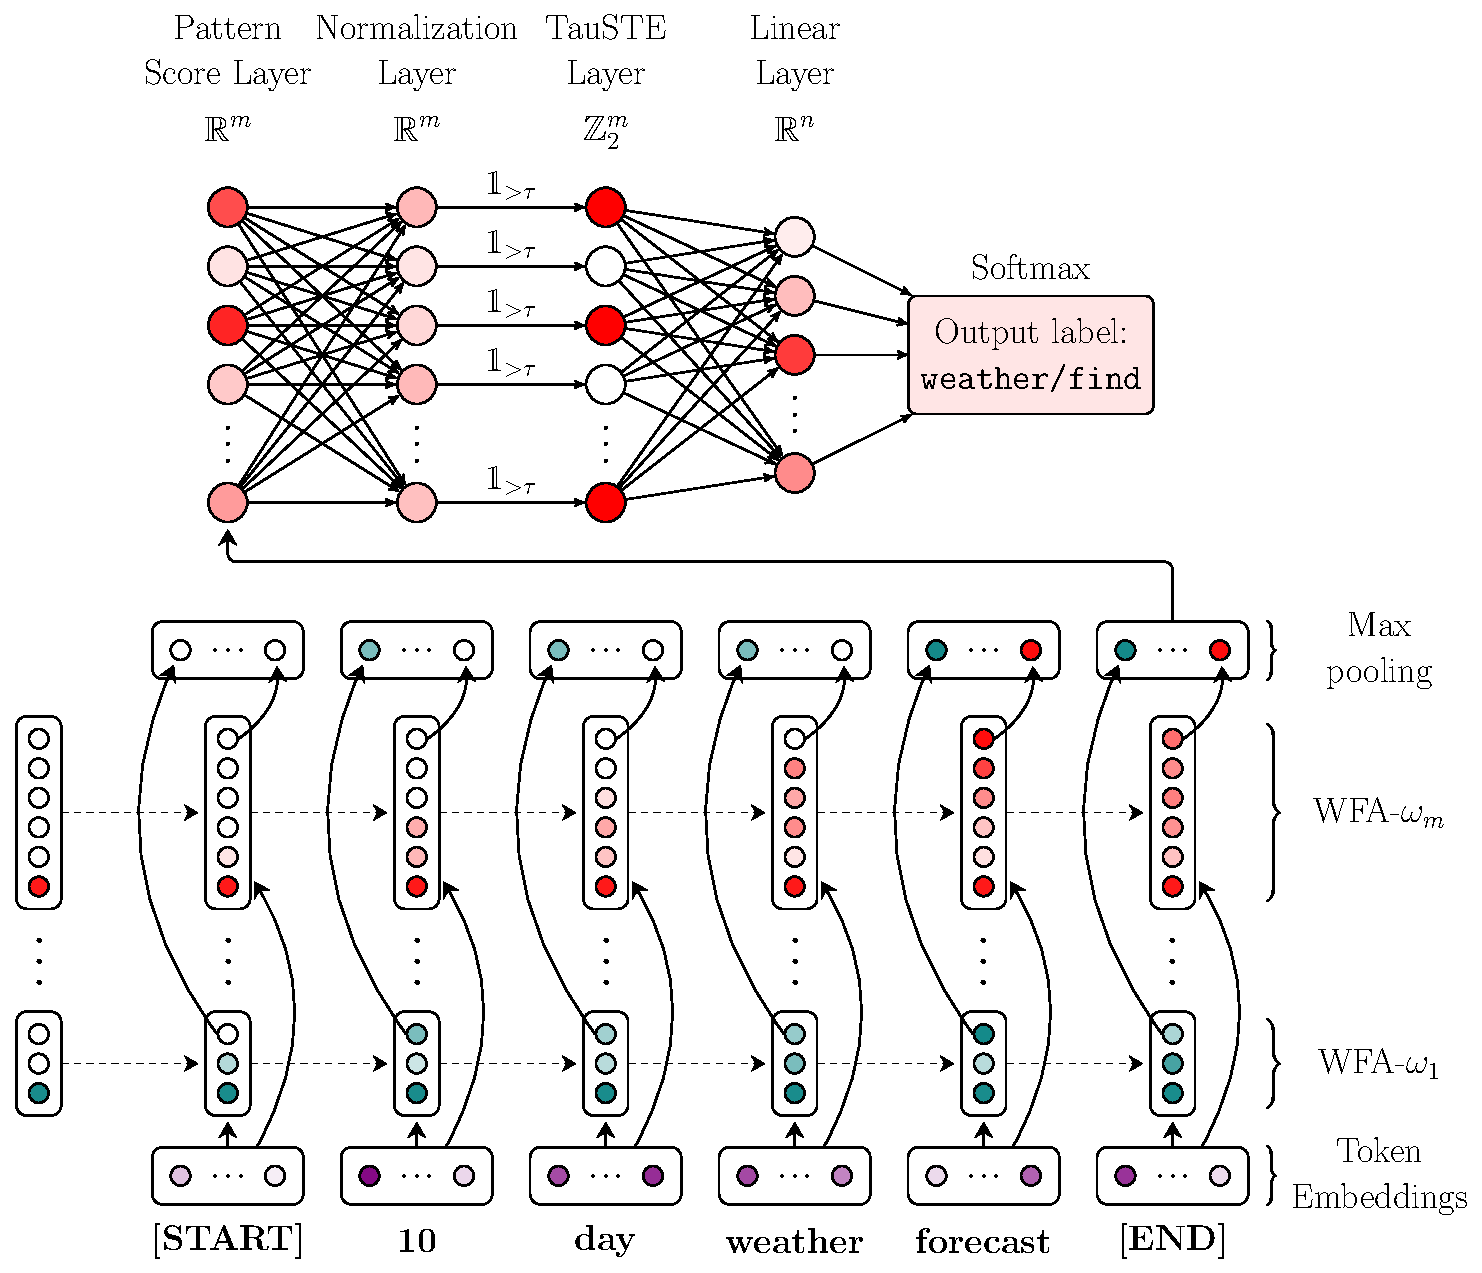
\includegraphics[width=8.5cm]{pdfs/generated/spp_computational_graph/main.pdf}
    \caption{SoPa++ computational graph; flow of graph is
      from bottom to top and left to right}
    \label{fig:spp_computational_graph}
  \end{figure}
\end{frame}

\begin{frame}
  \frametitle{SoPa++: Regular Expression (RE) proxy}
  \begin{figure}
    \centering
    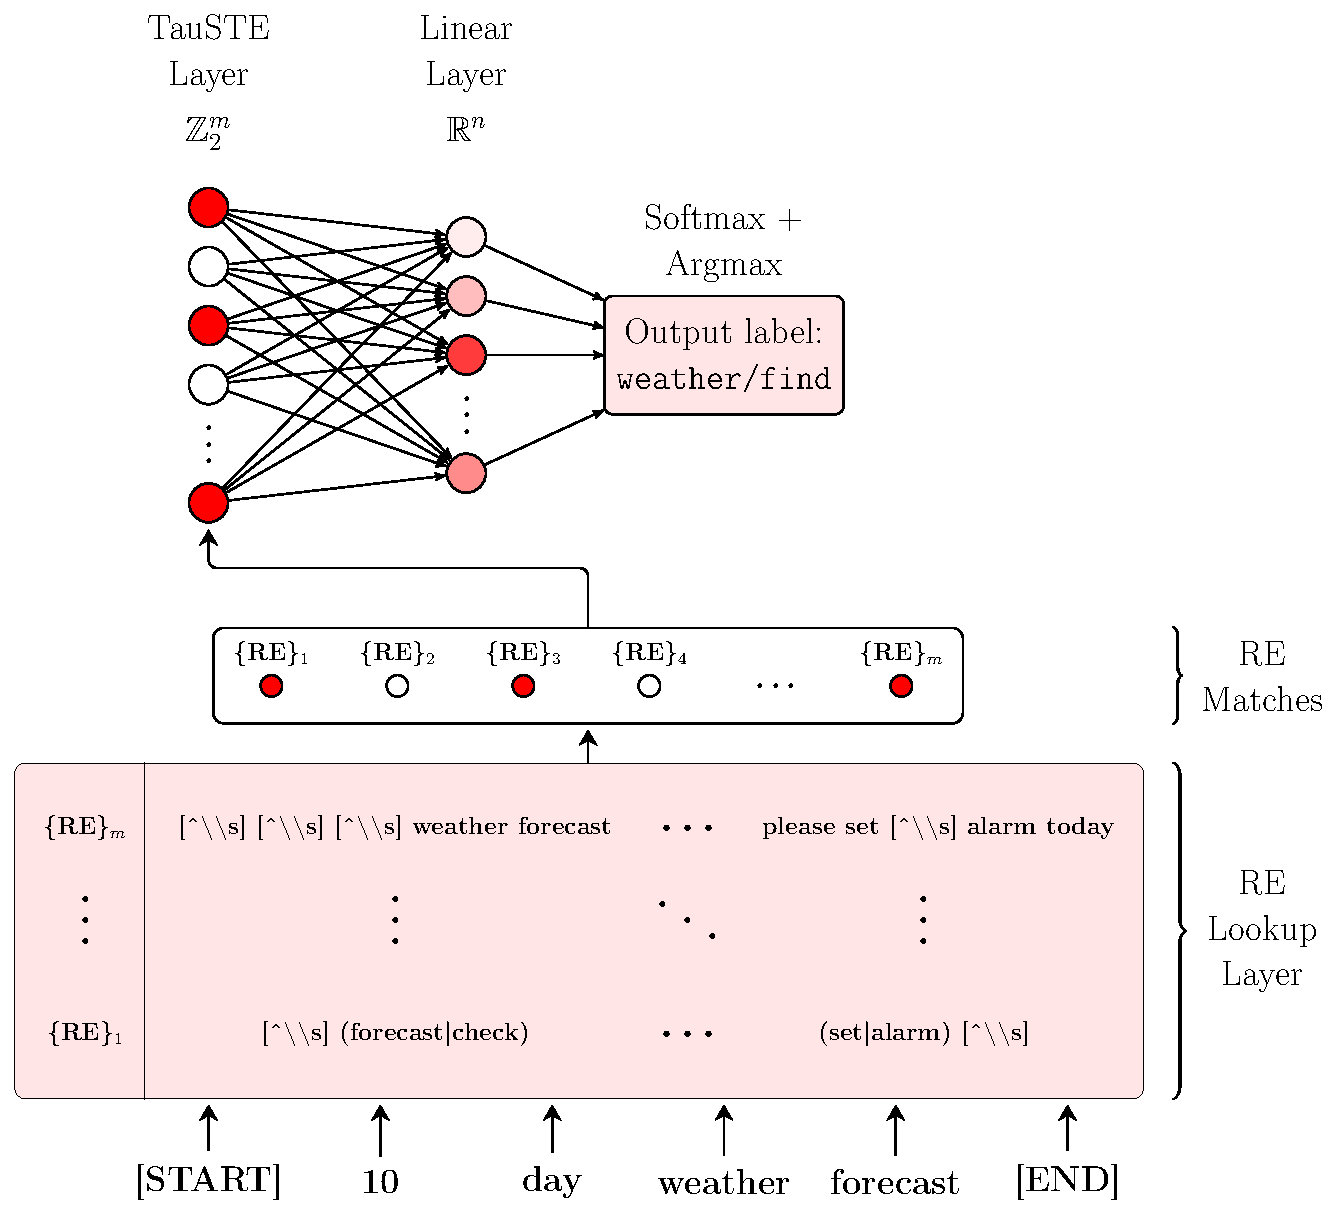
\includegraphics[width=8cm]{pdfs/generated/regex_computational_graph/main.pdf}
    \caption{RE proxy computational graph; flow of graph is
      from bottom to top and left to right}
    \label{fig:regex_computational_graph}
  \end{figure}
\end{frame}

\begin{frame}
  \frametitle{SoPa vs. SoPa++}
  \begin{table}[t!]
    \centering \def\arraystretch{1.5}
    \begin{tabular}{L{0.275\linewidth} L{0.3\linewidth} L{0.3\linewidth}}
      \toprule
      Characteristic & SoPa & SoPa++ \\
      \midrule
      Text casing & True-cased & Lower-cased \\ 
      Token embeddings & GloVe 840B 300-dimensions & GloVe 6B 300-dimensions \\
      \textbf{WFAs} & Linear-chain WFA's with $\epsilon$, self-loop and main-path transitions & Strict linear-chain WFA-$\omega$'s with $\omega$ and main-path transitions \\
      \textbf{Hidden layers} & Multi-layer perceptron after max-pooling & Layer normalization, TauSTE and linear transformation after max-pooling \\
      \textbf{Post-hoc explainability technique(s)} & Local explanations, feature relevance & Explanations by simplification \\
      \bottomrule
    \end{tabular}
    \caption{Summarized differences for SoPa vs. SoPa++}
    \label{tab:sopa_spp_comparison}
  \end{table}
\end{frame}

\begin{frame}
  \frametitle{Research Question 1: Performance}
  \uncover<2>{\begin{table}[t!]
    \centering
    \begin{tabular}{lll}
      \toprule
      Model size & Patterns hyperparameter $P$ & Parameter count \\
      \midrule
      Small & \texttt{6-10\_5-10\_4-10\_3-10} & 1,260,292 \\
      Medium & \texttt{6-25\_5-25\_4-25\_3-25} & 1,351,612  \\
      Large & \texttt{6-50\_5-50\_4-50\_3-50} & 1,503,812 \\
      \bottomrule
    \end{tabular}
    \caption{Three different SoPa++ model sizes used during training}
    \label{tab:model_types}
  \end{table}}
  \begin{itemize}
    \setlength\itemsep{1em}
    \uncover<1>{\item RQ 1: Does SoPa++ provide \textbf{competitive} performance?
    \item Competitive accuracy range: \textbf{96.6-99.5\%}
    \citep{schuster-etal-2019-cross-lingual,zhang2019joint,zhang-etal-2020-intent}}
    \uncover<2>{\item Upsampling minority classes to mitigate data imbalance
    \item Grid-search with three model sizes, varying $\tau$-thresholds: $\{0.00, 0.25, 0.50,
    0.75, 1.00\}$ and 10 random seed iterations
    \item $3 \times 5 \times 10 = 150$ model runs
    \item Evaluation and comparison on the test set}
  \end{itemize}
\end{frame}

\begin{frame}
  \frametitle{Research Question 2: Explanations}
  \begin{itemize}  
    \setlength\itemsep{1em}
    \uncover<1>{\item RQ 2: To what extent does SoPa++ contribute to \textbf{effective}
    explanations by simplification?
    \item Effective explanations by simplification requires \textbf{simpler model},
    \textbf{similar performance} and \textbf{maximizing resemblance} to
    antecedent
    \item Similar performance $\Rightarrow$ compare test set evaluations
    \item Maximum resemblance $\Rightarrow$ minimum distances}
    \uncover<2>{\item Softmax distance norm:
    \begin{equation*}
      \delta_{\sigma}(\bm{y}) = \left\Vert \bm{\sigma_{\mathcal{S}}}(\bm{y}) - \bm{\sigma_{\mathcal{R}}}(\bm{y}) \right\Vert_{2} = \sqrt{\sum^n_{i=1} (\sigma_{\mathcal{S}_i}(\bm{y}) - \sigma_{\mathcal{R}_i}(\bm{y}))^2} 
    \end{equation*}
    \item Binary misalignment rate:
    \begin{equation*}
      \delta_b(\bm{y}) = \dfrac{\left\Vert \bm{b_{\mathcal{S}}}(\bm{y}) - \bm{b_{\mathcal{R}}}(\bm{y}) \right\Vert_{1}}{dim(\bm{b_{\mathcal{S}}}(\bm{y}) - \bm{b_{\mathcal{R}}}(\bm{y}))} = \dfrac{\sum^n_{i=1} |b_{\mathcal{S}_i}(\bm{y}) - b_{\mathcal{R}_i}(\bm{y})|}{{dim(\bm{b_{\mathcal{S}}}(\bm{y}) - \bm{b_{\mathcal{R}}}(\bm{y}))}}
    \end{equation*}}
  \end{itemize}
\end{frame}

\begin{frame}
  \frametitle{Research Question 3: Relevance}
  \begin{itemize}
    \setlength\itemsep{2em}
    \uncover<1>{\item RQ 3: What \textbf{interesting and relevant} explanations can SoPa++
    provide?
    \item Open-ended question, can answer in different ways}
    \uncover<2>{\item Capitalize on the new linear layer $\Rightarrow$ allows for direct
    analysis of relative linear weights
    \item Sample REs from RE lookup layer corresponding to salient TauSTE
    neurons
    \item Analyze REs for interesting linguistic features and inductive biases}
  \end{itemize}
\end{frame}

\section{Results}
\section{Discussion}
\section{Conclusions}
\section{Future work}

\begin{frame}[allowframebreaks]
  \frametitle{Bibliography} \printbibliography[title = {Bibliography}]
\end{frame}

\end{document}
